\documentclass{article}

% Geometry package
\usepackage[a4paper, margin=0.5in]{geometry}

% Other packages
\usepackage{hyperref}
\usepackage{longtable}
\usepackage{tikz}
\usetikzlibrary{shapes, arrows}
\usepackage{float}

% Title
\renewcommand{\maketitle}{
  \begin{flushleft}
    ZC - University of Science and Technology
    \hfill Spring 2023 \\
    Communications \& Information Engineering Program
    \hfill Team: \textbf{ReflectoRay} \\
    CSCI 101: Introduction to Computer Science
  \end{flushleft}
  \begin{center}
    \LARGE Project Design
  \end{center}
  \begin{flushleft}
    Team: \textbf{ReflectoRay} \\
    Team Members: \\
    \textbf{
      \begin{tabular}{ccc}
        202201079 & SalahDin Ahmed Salh Rezk & \href{mailto:s-salahdin.rezk@zewailcity.edu.eg}{s-salahdin.rezk@zewailcity.edu.eg} \\
        202201293 & Ahmed Muhammad Abdullah & \href{mailto:s-ahmed.abdullah@zewailcity.edu.eg}{s-ahmed.abdullah@zewailcity.edu.eg} \\
        202201517 & Salah Mahmoud Gamal & \href{mailto:s-salah.gamal@zewailcity.edu.eg}{s-salah.gamal@zewailcity.edu.eg}
    \end{tabular} } \\
    Team Contact: \textbf{\href{mailto:s-salahdin.rezk@zewailcity.edu.eg}{s-salahdin.rezk@zewailcity.edu.eg}}
  \end{flushleft}
}

% Document
\begin{document}

% front matter
\maketitle

\begin{abstract}
  The Ray Reflection Simulation is a Python program that simulates the
  reflection of rays off mirrors. The simulation uses the Turtle graphics
  library to visualize the behavior of rays as they interact with mirrors,
  allowing users to explore principles of reflection and geometric optics.
  The project aims to provide an educational and interactive tool for
  understanding the principles of ray reflection. By allowing users to configure
  initial conditions and visualize the behavior of rays, the simulation promotes
  learning in the field of geometric optics.
\end{abstract}

\begin{longtable}{c|p{3.3cm}|p{3.3cm}|p{3cm}|p{1.5cm}}
  \bf Name & \bf Input & \bf Return & \bf Description & \bf Member \\
  \hline
  \texttt{parse\_arguments} & None & \texttt{argparse.Namespace} & Parse
  command line arguments. & Ahmed \\
  \hline
  \texttt{load\_initial\_conditions} & \texttt{file\_path: str} & \texttt{dict} & Load initial conditions from a JSON file. & Ahmed \\
  \hline
  \texttt{setup\_screen} & None & \texttt{turtle.Screen} & Set up the turtle
  screen for the simulation. & Salah \\
  \hline
  \texttt{draw\_mirrors} & \texttt{mirrors: list} & None & Draw mirrors on the turtle screen. & Salah \\
  \hline
  \texttt{create\_ray} & \texttt{angle: int, start: tuple, color: str} &
  \texttt{turtle.Turtle} & Create a turtle object representing a ray. &
  Salah \\
  \hline
  \texttt{create\_rays\_from\_sources} & \texttt{angles: list, sources:
  list} & \texttt{list} & Create rays from the sources. & Salah \\
  \hline
  \texttt{distance} & \texttt{point: tuple, line\_start: tuple, line\_end:
  tuple} & \texttt{float} & Calculate the distance between a point and a
  line. & Salah \\
  \hline
  \texttt{reflect\_ray} & \texttt{incident\_angle: float, line\_start:
  tuple, line\_end: tuple} & \texttt{float} & Calculate the reflection angle
  based on incident angle and mirror orientation. & SalahDin \\
  \hline
  \texttt{extend\_ray} & \texttt{ray: turtle.Turtle} & None & Extend the ray
  to simulate reflection. & SalahDin \\
  \hline
  \texttt{setup\_simulation} & \texttt{mirrors: list, sources: list, angles:
  list} & \texttt{turtle.Screen, list} & Set up the simulation with mirrors,
  sources, and angles. & SalahDin \\
  \hline
  \texttt{simulate\_rays} & \texttt{rays: list, mirrors: list} & None &
  Simulate the reflection of rays off mirrors. & SalahDin \\
  \hline
  \texttt{run\_simulation} & \texttt{screen: turtle.Screen, rays: list,
  mirrors: list, iterations: int, video: str, tmp: TemporaryDirectory} &
  None & Run the simulation with progress tracking and optional video
  recording. & SalahDin \\
  \hline
  \texttt{save\_image} & \texttt{screen: turtle.Screen, output: str} & None
                       & Save the screen as a PNG image. & Ahmed \\
                       \hline
  \texttt{convert\_eps\_to\_png} & \texttt{folder: str} & None & Convert EPS
  images in the input folder to PNG. & Ahmed \\
  \hline
  \texttt{save\_video} & \texttt{folder: str, output: str, fps: int, codec:
  str} & None & Save images in the input folder as a video. & Ahmed \\
  \hline
  \texttt{save\_output} & \texttt{screen: turtle.Screen, image: str, video:
  str, tmp: TemporaryDirectory} & None & Save the output as an image or
  video. & Ahmed \\
  \hline
  \texttt{main} & None & None & Main function to run the ray reflection
  simulation. & Salah \\
  \hline
  \caption{Functions Implementation}
\end{longtable}

\begin{figure}[H]
  \centering
  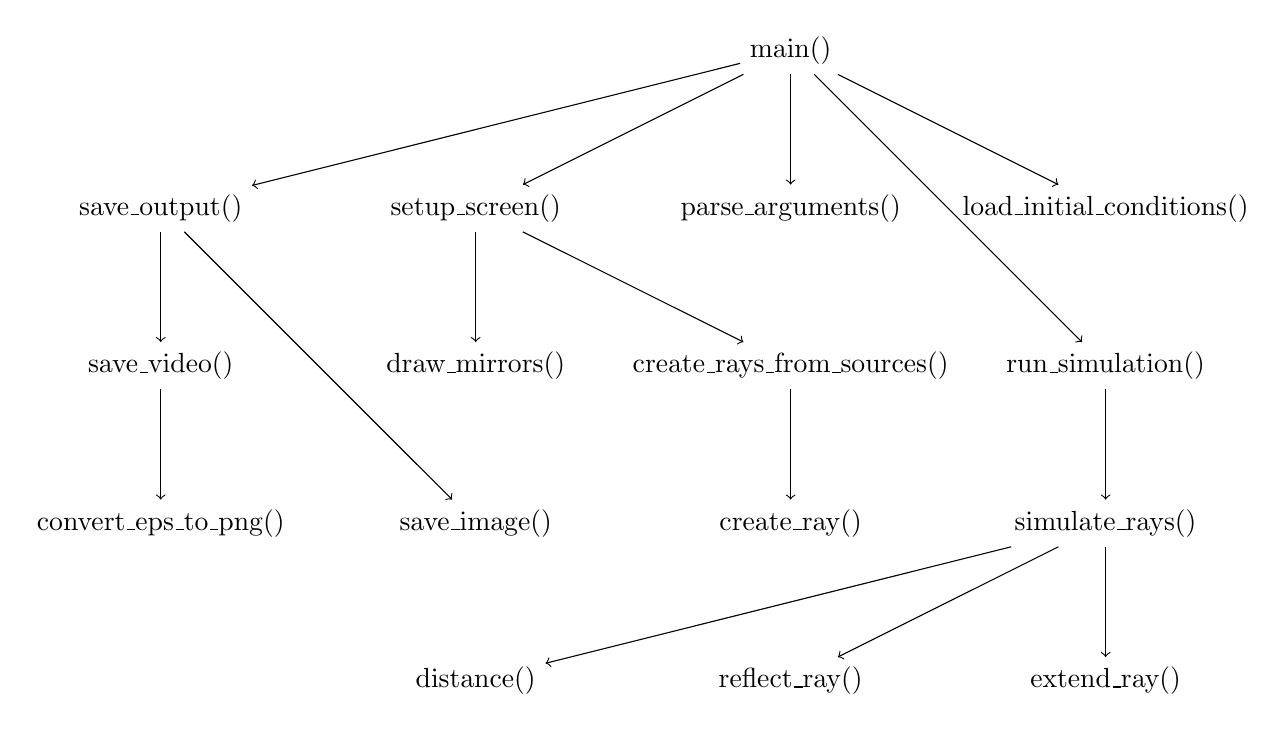
\begin{tikzpicture}[node distance=2cm, auto]
    % Nodes
    \node (main) {main()};
    \node (parse) [below of=main] {parse\_arguments()};
    \node (load) [right of=parse, xshift=2cm] {load\_initial\_conditions()};
    \node (setup) [left of=parse, xshift=-2cm] {setup\_screen()};
    \node (save) [left of=setup, xshift=-2cm] {save\_output()};
    \node (video) [below of=save] {save\_video()};
    \node (convert) [below of=video] {convert\_eps\_to\_png()};
    \node (draw) [below of=setup] {draw\_mirrors()};
    \node (image) [below of=draw] {save\_image()};
    \node (create) [right of=draw, xshift=2cm] {create\_rays\_from\_sources()};
    \node (ray) [below of=create] {create\_ray()};
    \node (run) [below of=load] {run\_simulation()};
    \node (sim) [below of=run] {simulate\_rays()};
    \node (ext) [below of=sim] {extend\_ray()};
    \node (ref) [left of=ext, xshift=-2cm] {reflect\_ray()};
    \node (dis) [left of=ref, xshift=-2cm] {distance()};

    % Arrows
    \draw [->] (main) -- (parse);
    \draw [->] (main) -- (load);
    \draw [->] (main) -- (setup);
    \draw [->] (setup) -- (draw);
    \draw [->] (setup) -- (create);
    \draw [->] (create) -- (ray);
    \draw [->] (main) -- (run);
    \draw [->] (run) -- (sim);
    \draw [->] (sim) -- (ext);
    \draw [->] (sim) -- (ref);
    \draw [->] (sim) -- (dis);
    \draw [->] (main) -- (save);
    \draw [->] (save) -- (image);
    \draw [->] (save) -- (video);
    \draw [->] (video) -- (convert);

  \end{tikzpicture}
  \caption{Flow Chart of Functions}
\end{figure}

\end{document}
